\chapter{Point Cloud Compression}
\label{ch:compression}
This Chapter present the last subject of the internship, \emph{point cloud compression}. Section~\ref{sc:spec-compression} gives a lead on the context bringing such need. Then, Section~\ref{sc:work-compression} mentions notable previously-published work on the subject. In Section~\ref{sc:custom-compression} we describe a custom arithmetic approach. The benchmark result highlights the relevance of Zip Compression to our objectives. Finally, Section~\ref{sc:integration}
discusses \emph{Zip compression} integration to \CC.

\section{Specifications}
\label{sc:spec-compression}

\subsection{Context}
As said in the introduction, \CC provides a cloud service for client not having performant machines. When a client submit a job, at some point, data uploading starts including the point cloud (if available\footnote{The reconstruction can also be made with photos.}). If the upload fails due to lost internet connection or any other reason, the upload restarts from scratch. Many point clouds are huge with a file size over $10$ GB, some of them more than $100$ GB. A Point cloud
easily becomes the biggest part of the data being upload to the cloud service. Therefore, reducing its size before uploading it, is a first good step toward better cloud services. This is where the scope of this work ends. A second step would probably be to find a way to send data through streaming with a recovery system on the cloud in case of fail.

This is how the need for \emph{Point Cloud Compression} emerged.

\subsection{Objective}
The method of compression must observe the following rules:
\begin{itemize}
  \item take as input any point cloud, provided it is static.
  \item being lossless,
  \item being able to compress several fields such as: point locations, normals, colors, intensity,
  \item compress the point cloud size ideally by two (2),
  \item have a reasonable compressing time such that the uploading time saved thanks to file size reduction is not lost during point cloud compression.
\end{itemize}

\section{Related work}
\label{sc:work-compression}
This section introduces different approach for point cloud compression. There is a need for clarification. The term \emph{point cloud compression} generally refers to ingenious representations of point clouds such that they take less space and can be easily loaded and used. However, for easy readability purposes we also use \emph{point cloud compression} to refer to simple arithmetic compression even if they are applied without no context of what is being compressed.

\cite{qsplat, schnabel, gumhold, zhang}. // FIXME\\
\cite{brotli, 7zip}

Dire que les compressions arithmétiques ont l'avantage de pouvoir compresser sans se soucier du décompressement, utilisation facile, optimisations géométriques...

\section{A bit-wise compression of point cloud}
\label{sc:custom-compression}
This section describes a custom point cloud compression. It is not exaclty a compression algorithm as it is just a packed representation of the same point cloud.It just ignores useless data reguardind the needed precision. Section~\ref{subsc:overview-packed} explains how this packed representation is obtained while Section~\ref{subsc:compression-benchmark} compares it with Brotli, 7Z (LZMA) and Zip, other arithmetic compression algorithms.

\subsection{Overview}
\label{subsc:overview-packed}


\subsection{Comparison with Brotli, 7Z and Zip}
\label{subsc:compression-benchmark}

\begin{sidewaysfigure}[t]
    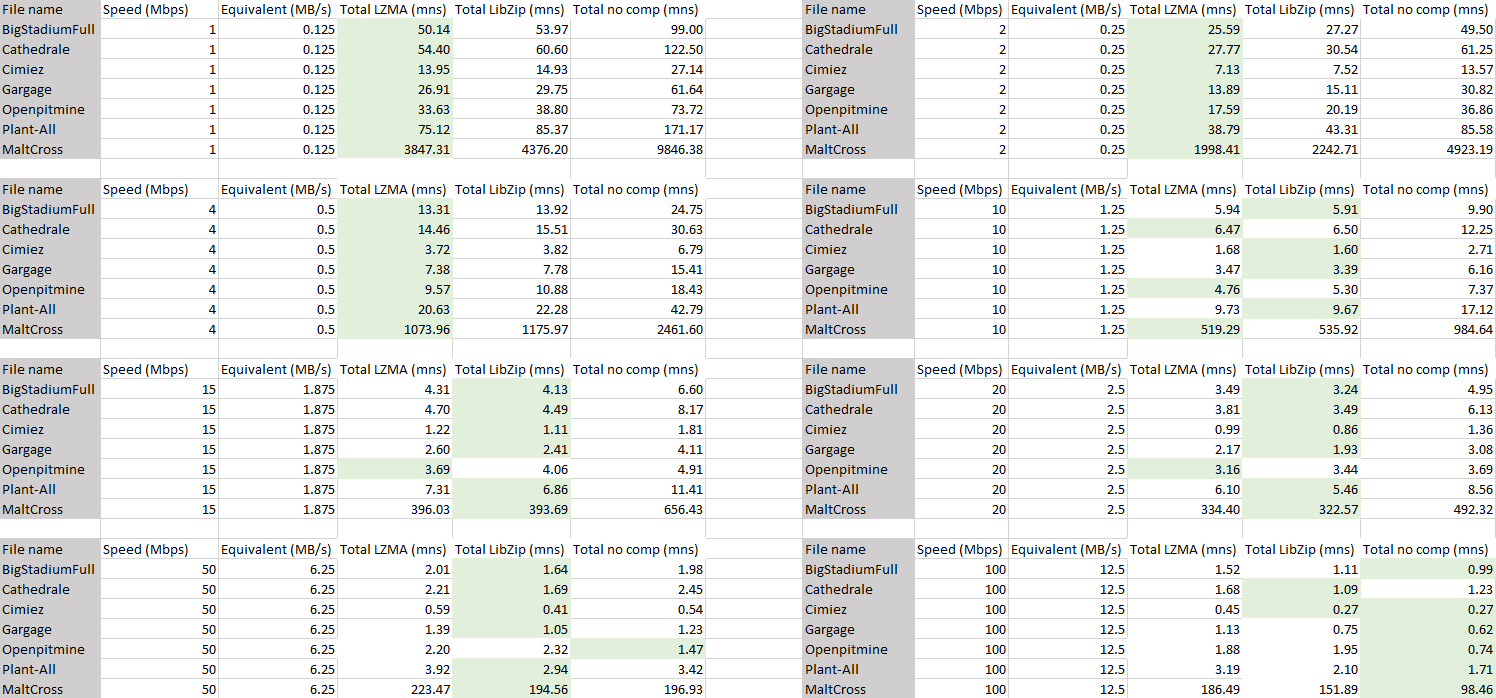
\includegraphics[width=\textwidth]{img/compare1.png}
    \caption{Caption in landscape to a figure in landscape.}
    \label{fig:compare-excel}
\end{sidewaysfigure}


\section{Integration of Zip compression}
\label{sc:integration}

\subsection{Code interface}
\begin{figure}
  \centering
  \begin{lstlisting}
  namespace Zip
  {
      bool compress(std::string const& inputPath, std::string const& outputPath,
              zip_progress_callback pf = nullptr, void* pProgressData = nullptr);

      bool decompress(std::string const& inputPath, std::string const& outputPath);
  }
  \end{lstlisting}
  \caption{Function using least-square to fit a line to the given set of points.}
  \label{fig:fitline}
\end{figure}


\subsection{\CC Software}
